\documentclass[twocolumn,german]{article}

% Die folgenden Definitionen sind i.w. identisch mit den
% Definitionen, die fuer Proceedings der IEEE vorgegeben werden.
% Papiere werden dort prinzipiell als article und zweispaltig
% gedruckt. Bei den IEEE-Definitionen werden Ueberschriften etwas
% kleiner und kompakter gesetzt (im Vergleich zu den
% Standard-Einstellungen, die sich mehr fuer 1-spaltigen Druck
% eignen. Wenn man das nicht mag, bleibt man bei den alten
% Definitionen. Bei den IEEE-Makros muss man unbequemerweise
% hinter jedem section-Kommando explizit \noindent angeben. 
% 
% Bei den IEEE-Definitionen muss leider hinter jeder
% Absatzueberschrift explizit ein \noindent stehen.

\makeatletter 
\def\@normalsize{\@setsize\normalsize{10pt}\xpt\@xpt
\abovedisplayskip 10pt plus2pt minus5pt\belowdisplayskip \abovedisplayskip
\abovedisplayshortskip \z@ plus3pt\belowdisplayshortskip 
6pt plus3pt minus3pt\let\@listi\@listI}
\def\subsize{\@setsize\subsize{12pt}\xipt\@xipt}
\def\section{\@startsection {section}{1}{\z@}
	{1.8ex plus 1ex minus .2ex} 
	{1.2ex plus .2ex \@afterindentfalse}
	{\large\bf}}
\def\subsection{\@startsection {subsection}{2}{\z@}
	{1.3ex plus 1ex}
	{.8ex plus .2ex \@afterindentfalse}
	{\subsize\bf}}
\def\paragraph{\@startsection {paragraph}{4}{\z@}
	{1.8ex plus .3ex}
	{-1em  \@afterindentfalse}
	{\normalsize\bf}}

\setlength{\textheight}{243mm}
\setlength{\columnsep}{6.5mm} %{2.0pc}
\setlength{\textwidth}{17cm}
\setlength{\parindent}{1pc}
\setlength{\parskip}{0.0cm}
\setlength{\topsep}{0.1cm}
\setlength{\partopsep}{0.0cm}
\setlength{\itemsep}{0.1cm}
\setlength{\parsep}{0.0cm}

% das folgende muss ggf. an die Einstellungen des 
% lokal vorhandenen Druckers angepasst werden.
\setlength{\topmargin}{-18mm} %original: -12mm
\setlength{\oddsidemargin}{-6mm}
\setlength{\evensidemargin}{-6mm}

\pagestyle{empty}
\thispagestyle{empty}

\baselineskip12pt


\pagestyle{empty}
\newcommand{\stt}{Soft\-ware\-tech\-nik-Trends}
%\raggedbottom

%\usepackage{flushend}
\usepackage[T1]{fontenc}
\usepackage[utf8]{inputenc}
\usepackage[ngerman,english]{babel}
\usepackage{graphicx}
\usepackage{tikz}
%\usepackage[backend=biber, style=apa, url=false]{biblatex}
%\addbibresource{vise.bib}
%\usepackage{hyperref}
%% Define a new field format for the URL/DOI to create a hidden link
%\DeclareFieldFormat{url}{%
%  \iffieldundef{url}%
%    {}%
%    {\href{\thefield{url}}{#1}}%
%}
\usepackage{hyperref}
\usepackage{cleveref}
\usepackage{framed}
\usepackage{listings}
\usepackage{paralist}
\usepackage{xcolor}
\usepackage{amssymb}

\newcommand{\todo}[1]{} %{{\small \textcolor{red}{TODO: #1}}}

\usepackage{etoolbox}
\patchcmd\thebibliography
 {\labelsep}
 {\labelsep\itemsep=-5pt\relax}
 {}
 {\typeout{Couldn't patch the command}}

\begin{document}
\setlength{\belowcaptionskip}{-10pt}
\twocolumn[{
\Large
\center{From Vibe to Vise Coding: Addressing the AI-Generated Code Quality Crisis}
%\center{Vise Coding: High-quality, sustainable AI-assisted software development}
\vspace{3mm}
\normalsize
\center{David Faragó, \href{mailto:drdavidfarago@gmail.com}{drdavidfarago@gmail.com}}
\vspace{3mm}
\slshape
}]

\section*{Abstract}
Current news claims that AI is replacing software developers~\cite{RJ25,KT25,ET25}.
However, such proclamations may primarily serve corporate narratives (like justifying layoffs or promoting AI products) rather than reflect reality.
We examine data on AI adoption and its effects, revealing that AI-assisted software development (``AI coding'' for short) improves,
but software engineering is far from full automation: 
The current hype often fails to distinguish between what large language models (LLMs) can and cannot do effectively.
This lack of nuance has led to AI coding practices that produce code unsuitable for production environments and maintenance.
%This problem culminates in ``Vibe Coding'', i.e. blindly accepting AI-generated code suggestions with no understanding or review.
Objective data signals that this kind of AI coding will lead to a software quality crisis.
The popularity of ``Vibe Coding'' -- blindly accepting AI's suggestions with no understanding or review -- aggravates the downward spiral:
more and more software security holes~\cite{HP25,CW25}, buggy behavior~\cite{Liu24}, performance decrease~\cite{SL24},
%and even whole projects going under [TODO:GB25,MR25,MS25,SV25b].
leading to outages~\cite{FJ24} and data loss~\cite{BN25}.
In response to these concerns, we introduce ``Vise Coding'', a term coined immediately after ``Vibe Coding'' emerged \cite{DF25},
which advocates for a more disciplined integration of AI:
like a craftsman's vise, documentation and process guides and checks the LLM to produce clean, production-ready code.

This paper firstly presents alarming data about the emerging software quality crisis,
then introduces Vise Coding as a solution: we detail its process, explain the necessary context engineering,
and provide an evaluation that demonstrates both the significant benefits of Vise Coding,
but also the limits of current AI coding.

Keywords: {\em LLM-based coding agents, AI-assisted coding, software quality, Vibe coding, Vise coding}

\section{Introduction}

LLMs became popular with GPT-3 in 2020;
their integration into software development started with GitHub Copilot in 2021 (see Fig.~\ref{fig:statusquo}). 
Unlike rule-based tools limited to single-line completions, Copilot generates complete method implementations.
GitHub Copilot Experimental Chat, introduced in 2022,
brought in-context learning for flexible code generation and code base queries. 
Subsequently, numerous tools emerged, offering similar and extended capabilities for
AI-assisted software development, hereon referred to as ``AI coding''.

Due to the tools' power and flexibility, they can be applied in various ways.
In February 2024, Andrej Karpathy introduced the term ``Vibe Coding'' for the most extreme approach of
``always accept all [of AI's code suggestions], don't read the diffs anymore, and just work around a bug
or ask for random changes until it goes away''~\cite{AK25}.
As this leads to ``write-only'' code, i.e. not readable, maintainable, or improvable code,
David Farag\'{o} proposed as counterpart ``Vise Coding'' a few weeks later,  
which preserves software craftsmanship principles when applying AI coding.
While the term Vise Coding is gaining traction in Germany~\cite{URL:ViseWikipediaDe},
it has not seen similar adoption internationally.
Nevertheless, Andrej Karpathy has later acknowledged the necessity of upholding
specific software craftsmanship principles when applying AI coding for real-world software~\cite{AK25c,AK25b}.

This paper firstly examines the status quo of AI coding,
demonstrating how practices that tend toward Vibe Coding are driving the industry toward a software quality crisis. 
Then Vise Coding is introduced as a systematic countermeasure, followed by its evaluation and conclusions.

\section{Software Development Status Quo}

\begin{figure}[hbt!]
  \vspace{-4mm}
  \hspace{-3mm}
  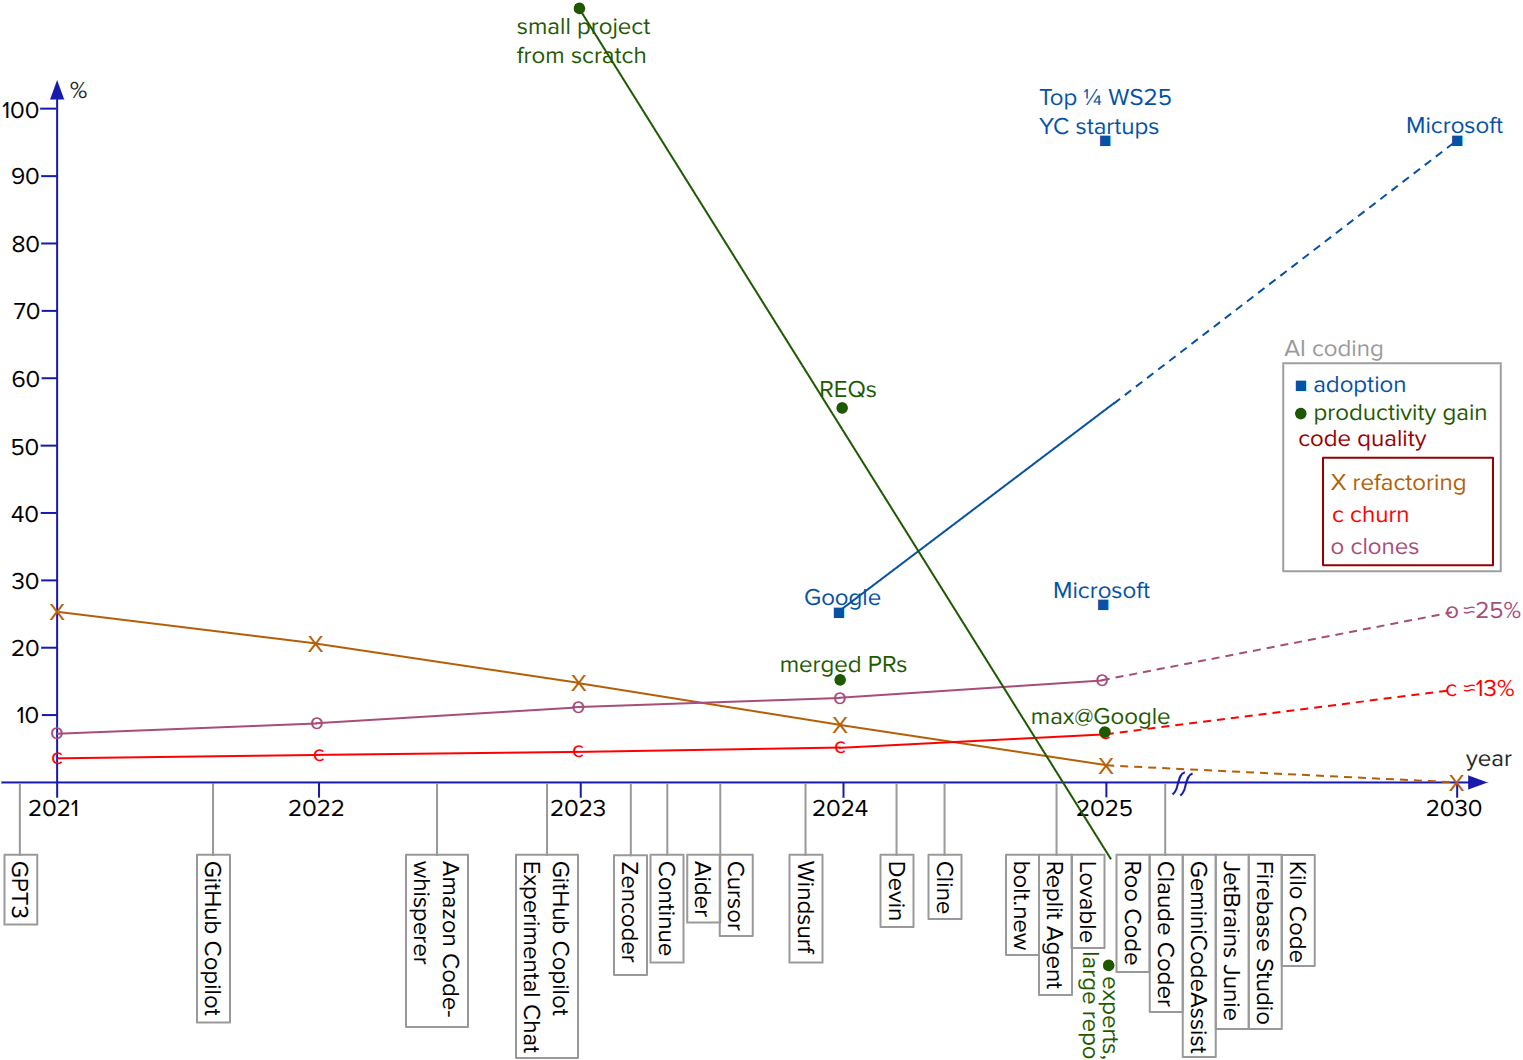
\includegraphics[width=0.49\textwidth]{figures/allStats_v4}
  \vspace{-7mm}
\caption{Status quo and trends of AI coding: high adoption, low productivity and quality}
\label{fig:statusquo}
\end{figure}

The {\color{blue}$\blacksquare$} plot in Fig.~\ref{fig:statusquo} depicts
at which rate AI coding is being adopted in industry:
\begin{compactitem}
\item Google, known for its rigorous software metrics,
  reported that over 25\% of their software was written by AI in 2024~\cite{RA24}
\item Microsoft reports similar numbers for 2025: 20\% to 30\%~\cite{MZ25}
\item for 2030, Microsoft's CEO predicts 95\% of its code being generated by AI~\cite{MG25}
\item the 95\% threshold has already been reached by the top 25\% of Y-Combinator startups
  founded in the winter 2024 to 2025~\cite{IM25}.
\end{compactitem}
So AI coding adoption has a steep increase; its popularity is also reflected by the number of AI coding tools and the company's investments. 
While measuring adoption is easy, this is harder for its productivity gain, and there are only a few thorough analyses, depicted by the {\color{green}$\bullet$} plot:
\begin{compactitem}
\item in 2023, \cite{peng23} measured that AI coding a small software project from scratch
  reduces the required time from 161 to 71 minutes on average, corresponding to a productivity gain of 127\%
\item in 2024, \cite{TW24} measured a 65\% increase in the number of implemented requirements with the help of AI coding,
  \cite{KC24} a 15\% increase in the number of merged PRs
\item in 2025, \cite{DORA25} reported an increase of 2.1\% per 25 percentage points AI adoption, so maximally 8.4\%, while
  \cite{JB25} measured that expert developers have a 19\% slowdown for AI coding on large and complex repositories,
  compared to coding without AI.
\end{compactitem}
While these papers did not use the same metrics to measure productivity gains,
they show a severe downward trend or correction over the years.
A main cause for the reduced productivity gains is a strong reduction of software quality
with the adoption of AI coding, as measured on repository operations by \cite{WH25}:
\begin{compactitem}
\item the {\color{orange}x} plot shows that refactorings (measured via moved code operations) reduce yearly by 5 percentage points; if the trend continues, there will be next to no refactorings by 2026
\item the {\color{red}c} plot shows code churn, i.e. code that was either incomplete or erroneous when committed; a projection of the yearly increase of 1.2 percentage points will lead to 13\% of all repository operations being code churn by 2030
\item the {\color{purple}o} plot shows committed code clones; projecting the yearly increase of 2 percentage points will lead to 25\% of all repository operations introducing clones.
\end{compactitem}
Though there are more aspects to code quality, minimal refactorings combined with high code churn and clones 
are strong indicators of the low code quality that AI coding produces.
But there are many further common quality issues from AI coding, e.g. dead code,
implementation details drifting away from documentation,
and workarounds layered on top of bugs or undesired behavior instead of real fixes. 
Overall, Fig.~\ref{fig:statusquo} shows that AI coding has only short-term productivity gains at the cost of quality.
As low code quality and technical debt is accumulated rapidly with each iteration, understandability, readability, and maintainability is impaired, thereby impeding long-term productivity (see Fig.~\ref{fig:vibevise}). This is acceptable for prototypes, but not for production code you need to work with longer~\cite{AO25}.

\section{Vise Coding}

Significant efforts focus on rectifying quality issues in AI-generated code~\cite{URL:payasyoucode,URL:pragmaticcoders,URL:SECVAIB}.
However, fixing bugs, security vulnerabilities, and non-idiomatic patterns at later development phases is costly and unreliable.
Shifting left by intervening at the moment of AI's code generation to prevent or correct errors is a more effective approach\footnote{Improving LLM's ability to reliably generate correct code would be an even earlier phase, but in generality, this remains being a challenge~\cite{KH25,JB25,PL25,MH25,PS25,RS25}}.
Vise Coding introduces guardrails so that the LLM produces better code, tests, and documentation. 
Like a craftsman's vise that holds work steady while precision tools are applied,
Vise Coding uses comprehensive documentation and processes to constrain, guide, and filter the LLM's output.

\subsection{Product Requirements Documents}

Documentation becomes a first class citizen again for Vise Coding and
can function as a Product Requirements Document (PRD),
which is an up-to-date document defining a product's requirements,
including its purpose, features, functionality, and behavior to ensure clarity and alignment between client and supplier. 
PRDs used for AI coding are often also termed Prompt Requirements Document and
contain additional information, such as associated (sub-)tasks and priorities (similar to the data in issue trackers),
as well as organizational requirements, processes, and best practices (e.g. ``write code that takes dev, test, and prod into account'').
(BDD-style) test cases also function as guardrail and as exit criteria
and can be considered part of the code or the PRD.
We call the part of the PRD that is persisted for re-use over multiple coding sessions the persistent PRD, 
the other part temporary PRD, which mostly contains information only relevant to the current session.
The PRD is the craftsman's vise, the client is the human, and the supplier the LLM.

\subsection{Vise Coding Process}

The Vise Coding process iteratively updates the code and the PRD with the help of software development best practices and AI (see Fig.~\ref{fig:process}):
\begin{compactenum}[(a)]
\item add or extend the PRD for the code to be generated or modified\label{item:a} 
\item make small, high-quality code changes that are easy to review and verify\label{item:b}
\item update the persistent PRD accordingly.\label{item:c}
\end{compactenum}

In \ref{item:a}, the AI chat serves as temporary PRD and as orchestration mechanism.
For this, many AI coding tools offer a plan mode of chatting prior to code generation. 
\ref{item:b} retains software craftsmanship principles -- the professional responsibility to produce not only working software,
but also clean, well-crafted, well-tested, and reviewed software and documentation,
enabling continuous value addition and improvement.
\ref{item:c} should be performed at minimum at session completion,
but more frequent updates often yield superior solutions.
Of course changes to the persistent PRD are reviewed, too.

\begin{figure}[hbt!]
  \begin{center}
  \vspace{-4mm}
  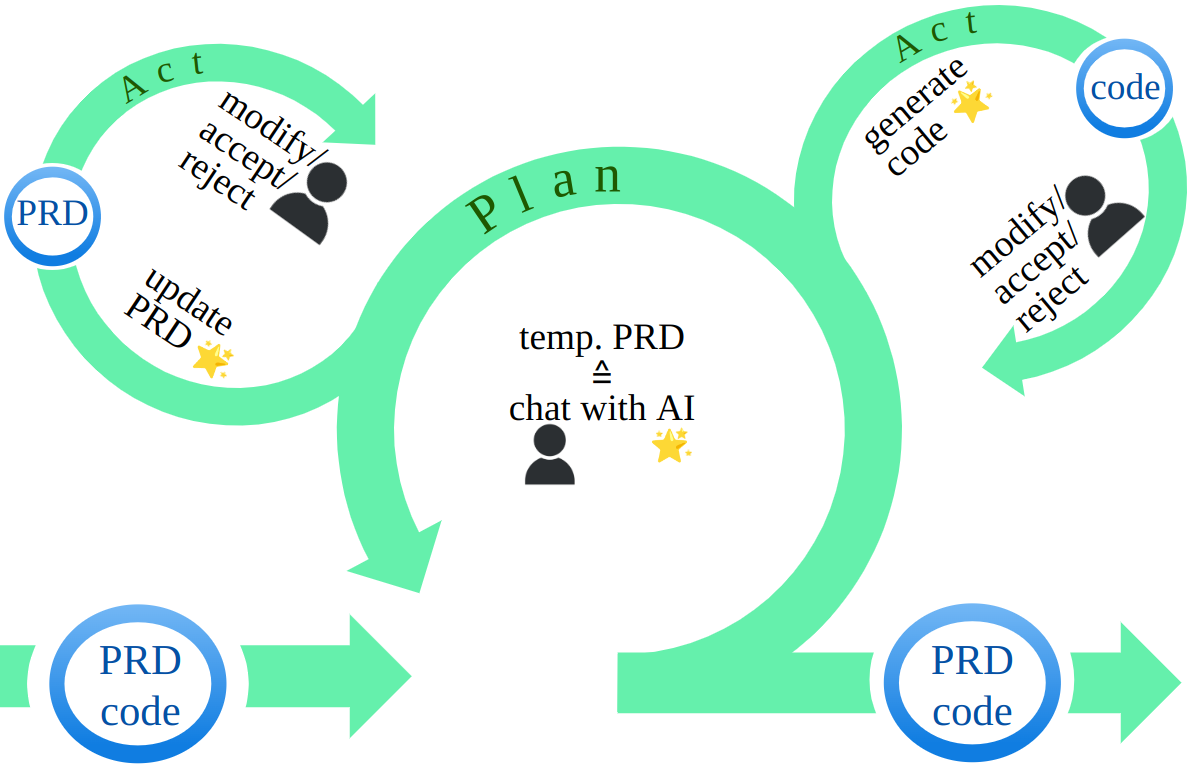
\includegraphics[width=0.45\textwidth]{figures/vise_process_v2}
  \vspace{-4mm}
\caption{Iterative Vise Coding process}
\label{fig:process}
\end{center}
\end{figure}

\subsection{Context Engineering}

Several AI coding tools introduced features to effectively manage organization- and project-dependent persistent PRDs:
%GitHub Copilot Experimental Chat (Nov. 2023),
Cursor Rules (April 2024), \lstinline|copilot-instructons.md| (Nov. 2024), Cline Custom Instructions and \lstinline|.clinerules| (Feb. 2025).

AI is also used for generating PRDs, e.g. by:
\begin{compactitem}
\item chatprd.ai (March 2024), a PRD generator, but without direct integration into an AI coding tool
\item Cline Memory Bank (Feb. 2025), which automatically generates persistent PRDs from existing code and documentation
\item MCP servers~\cite{URL:mcp}, which enable AI coding tools to connect to tools/resources/data,
  including filesystem-mcp for project structure analysis, git-mcp for repository context, Mem0, Knowledge Graph Memory, and Context7 for persistent knowledge.
\end{compactitem}
MCP servers are recreating established PRD management practices within AI coding,
enabling seamless integration with enterprise tools (Jira, Confluence, Notion) for automated PRD extraction,
version control synchronization, traceability, and cross-repo support.

Since an AI coding session can have many turns, the LLM's context can become huge, which hurts its effectiveness~\cite{KH25}.
To keep the context tidy, there are two common context engineering practices to manage and modularize sessions
(see Fig.~\ref{fig:pipelinesubtask}):
\begin{compactitem}
\item pipeline, e.g. using Cline's Plan and then Act mode or its slash commands: 
\lstinline|\newrule| to persist some part from the temp. PRD;
\lstinline|\newtask| to hand-off the next subtask to a new session by preparing a corresponding temp. PRD;
\lstinline|\deep-planning| to have a pipeline of code investigation, chat, and planning,
and then a hand-off to a coding subtask;
\lstinline|\smol| to remove the noise from the temp. PRD but continue the session;
\lstinline|\workflowname| to iterate over a specific workflow in individual sessions
\item subroutines, where an orchestrator session decides which subroutine to call in which order.
The orchestrator is kept tidy since subroutines execute in an own session and only return a summary to the orchestrator.
Roo Code's Boomerang Tasks implement this, but you need to define your subroutines (called modes) in advance,
e.g. for testing you could specify
  \lstinline|write-tests-for-new-feature|, \lstinline|fix-tests-true-positive|, \lstinline|write-tests-for-broken-code|,
  \lstinline|fix-tests-false-positive|, \lstinline|write-tests-for-correct-code|.
\end{compactitem}
Further context engineering features are available as MCP servers, e.g. Shrimp Task Manager and Sequential Thinking MAS.

\begin{figure}[hbt!]
  \vspace{-2mm}
  \hspace{-3mm}
  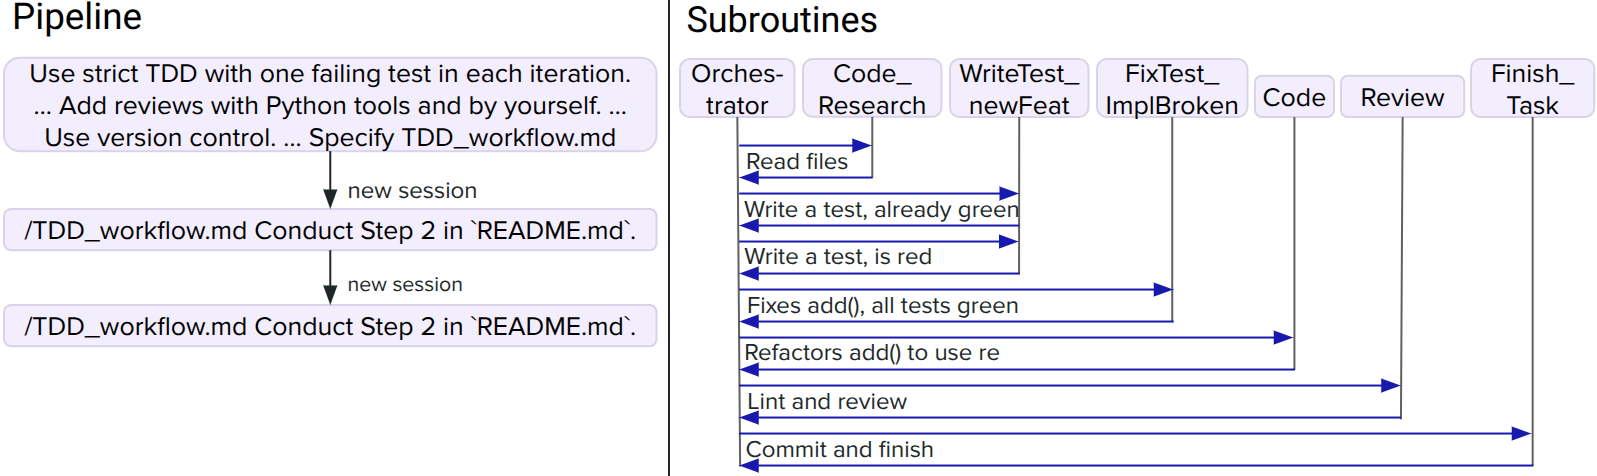
\includegraphics[width=0.49\textwidth]{figures/pipeline_vs_subtask_v3}
  \vspace{-8mm}
\caption{Modularization into multiple sessions}
\label{fig:pipelinesubtask}
\end{figure}

\section{Evaluation}

Since AI coding has so many parameters (repo size, session length, programming language, AI coding tool, LLM,
%LLM's thinking amount,
PRD, context engineering, MCP servers)
and the LLM's effectiveness differs for seemingly similar problems (Jagged Technology Frontier)~\cite{FD23},
a statistically sound evaluation would need to be based on thousands of AI coding sessions, which we do not yet have.
Thus these evaluations need to be taken with a grain of salt.

\subsection{AI coding tool, LLM, context engineering}
\label{sec:gradedsessions}

Fig.~\ref{fig:toolsmodels} presents David Farag\'{o}'s personal Vise Coding sessions from February 19th to May 21st that have been manually graded in a very critical way.
It shows the huge variance, which is likely due to the latent dimensions and the Jagged Technology Frontier.
Consistently good (but not very good) results were achieved with Cline with Memory Bank and Gemini 2.5 Pro.

\begin{figure}[hbt!]
    \vspace{-1mm}
    \hspace{-3mm}
  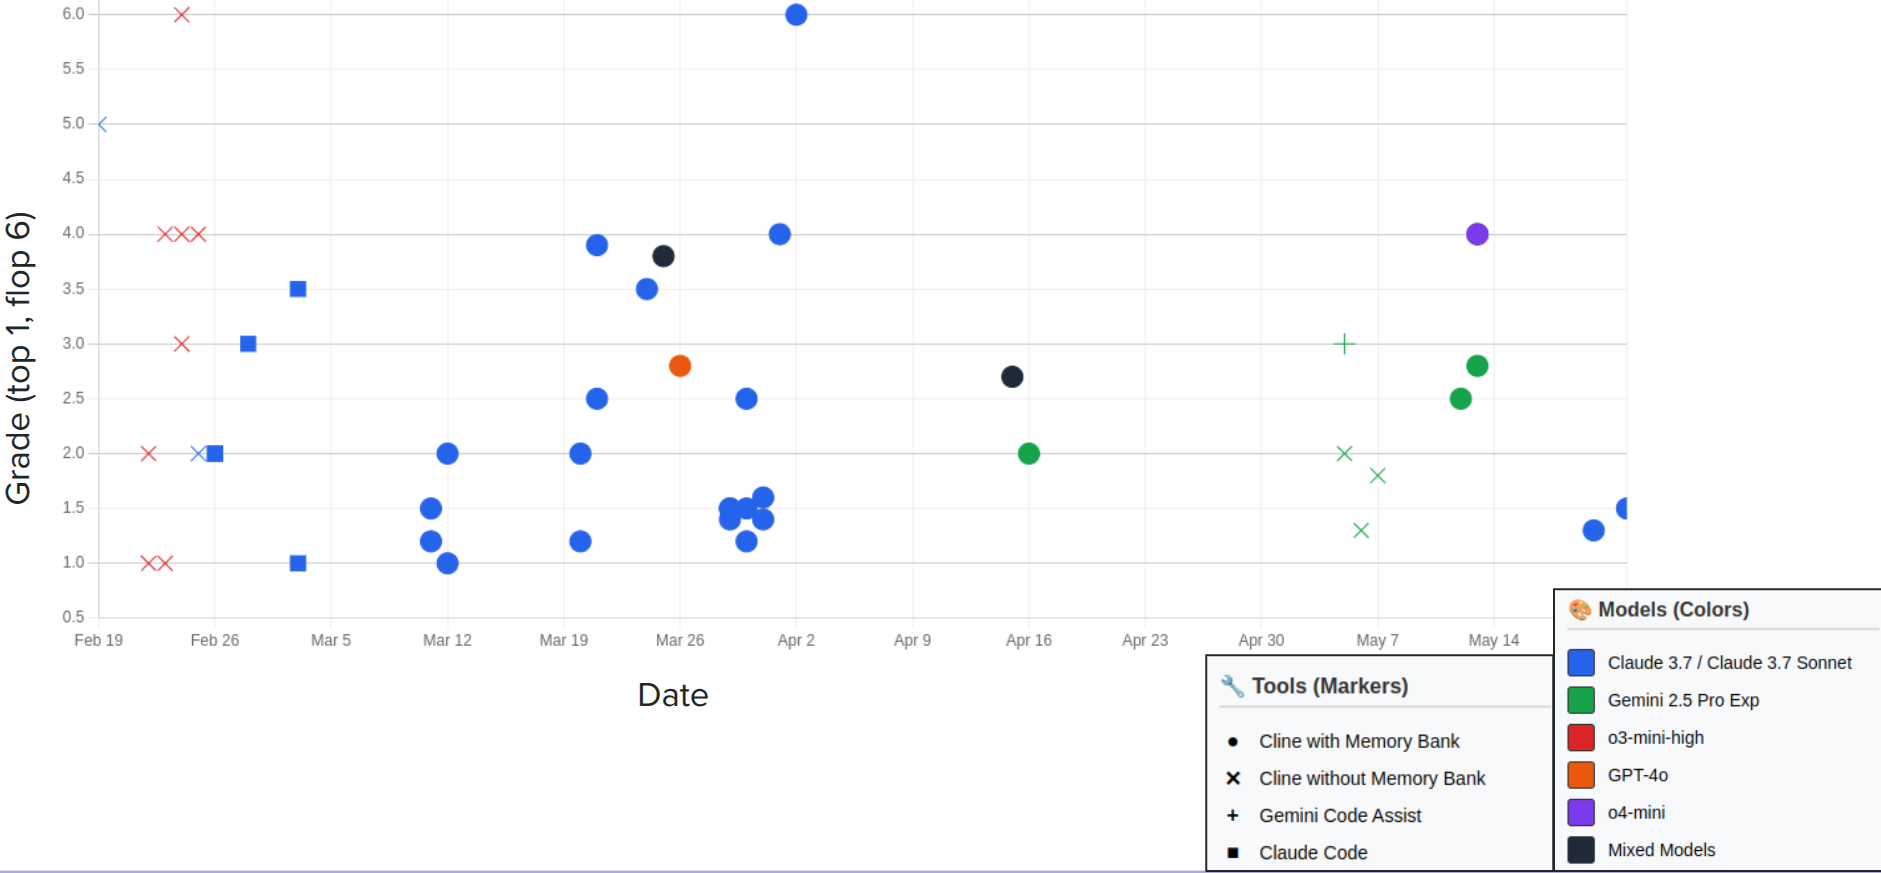
\includegraphics[width=0.49\textwidth]{figures/tools_models_v1}
  \vspace{-7mm}
\caption{Graded sessions for various tools and models}
\label{fig:toolsmodels}
\end{figure}

\subsection{Context Engineering}

There are many aspects to context engineering. We consider pipelines vs subroutines, and how good context engineering can cope with context size.

%LAYOUT HACK, should be at the end of this subsection
\begin{figure*}[hbt!]
  \begin{center}
  \vspace{-1mm}
  \fbox{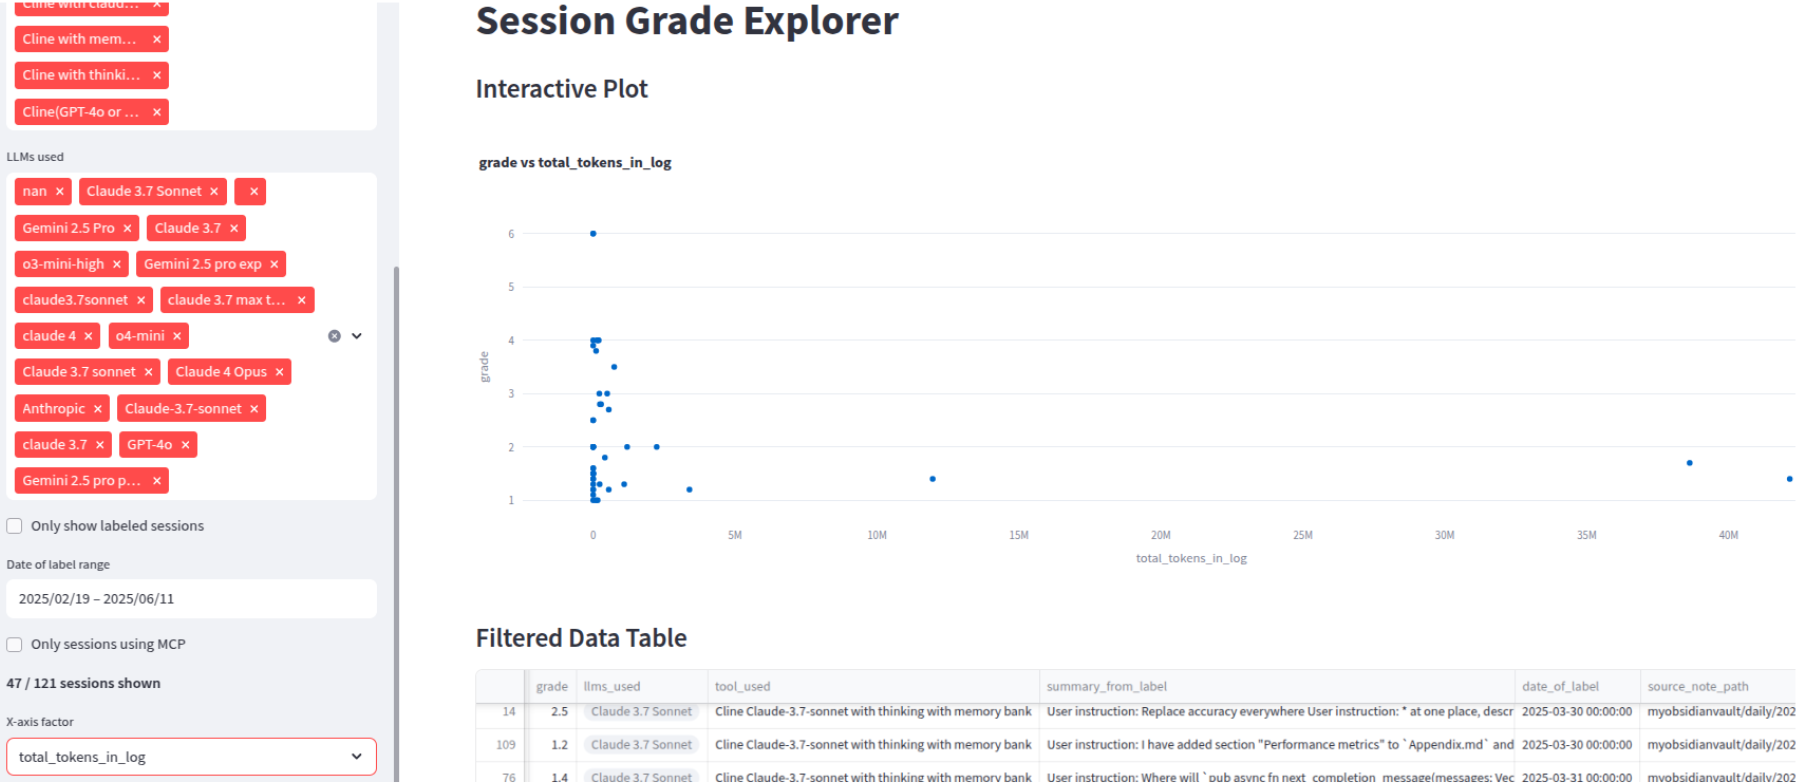
\includegraphics[width=0.98\textwidth]{figures/session_grade_explorer_v1}}
  \vspace{-5mm}
\caption{Grades depending on total session tokens}
\label{fig:evaltool}
\end{center}
\end{figure*}

For pipelines, you can decide dynamically when to shrink your context, when to start a new task, or when to create and iteratively execute a workflow.
This gives great flexibility. For subroutines, you have less flexibility because you need to pre-define your subroutines. You usually have 5 to 20 that you can highly optimize. If the are suitable for your task, you get reliably better results then with pipelines. 
Fig.~\ref{fig:pipelinesubtask} gives an example for the \lstinline|string-calculator-kata|, where subroutines led to better results at half the price.

Fig.~\ref{fig:evaltool} plots the critically graded Vise Coding sessions (see Sec.\ref{sec:gradedsessions}) depending on the total tokens in the whole session:
the larger the session, the better the grades, showing that adding all the relevant context helps in Vise Coding, and that context engineering can cope with large context.


\subsection{Vibe Coding vs Vise Coding}

This section gives an exemplary evaluation of Vibe Coding vs Vise Coding on an Extract-Transform-Load project for creating an interactive exploration tool
for the critically graded Vise Coding sessions, see Fig.~\ref{fig:evaltool}. Vise Coding has been performed with Cline, Vibe Coding with Google Jules,
but the results are representative.

Extract: to extract data, only Cline was used, because Jules does not offer MCP tools. Cline used an Obsidian MCP server to extract grades
and packaged them with the session log file.
Without slash commands, this took about 6 hours with little intervention for iterating through the sessions to be extracted,
resulted in 850k context size and therefore cost 80\$. Using instead workflows was much cheaper,
but required repeated triggering of the workflow. Cline's extract was graded 1.6.

Transform: to transform the extracted data into a table for later exploration,
Cline produces slightly redundant code with 1 bug that was easily fixed.
It required 753k context size, about 2 hours, and cost 10\$. Hence it was graded 2.1.
Jules produces within 1 hour without any intervention code that is too complex, had a lot of bugs and partly unnecessary. 
It was graded 4.9

Data visualization GUI: Cline produces a GUI that was interactive, robust, and usable, but visually ugly.
It required 29k context size, about 1 hour, and cost 13\$. Hence it was graded 2.2.
For Jules, the table produced by Cline's transform was used, because it was cleaner and contained more data.
Jules was unable to complete the task: the code contained lots of \lstinline|TODO|s,
did not make sensible visualizations and crashed on first interaction.
It required 1 hour without any intervention. Hence it was graded 5.4.

\section{Conclusion}
Vise Coding does not compromise software quality.
It makes use of AI to accelerate the development (see Figure \ref{fig:vibevise}),
but humans stay tightly in the loop.
%As AI agents evolve to reliably generate PRDs and correct code,
%the degree of autonomy might successively be increased.
As the reliability of AI agents in generating suitable PRDs and correct code increases, so too can their degree of autonomy.

\begin{figure}[hbt!]
  \begin{center}
  \vspace{-2mm}
  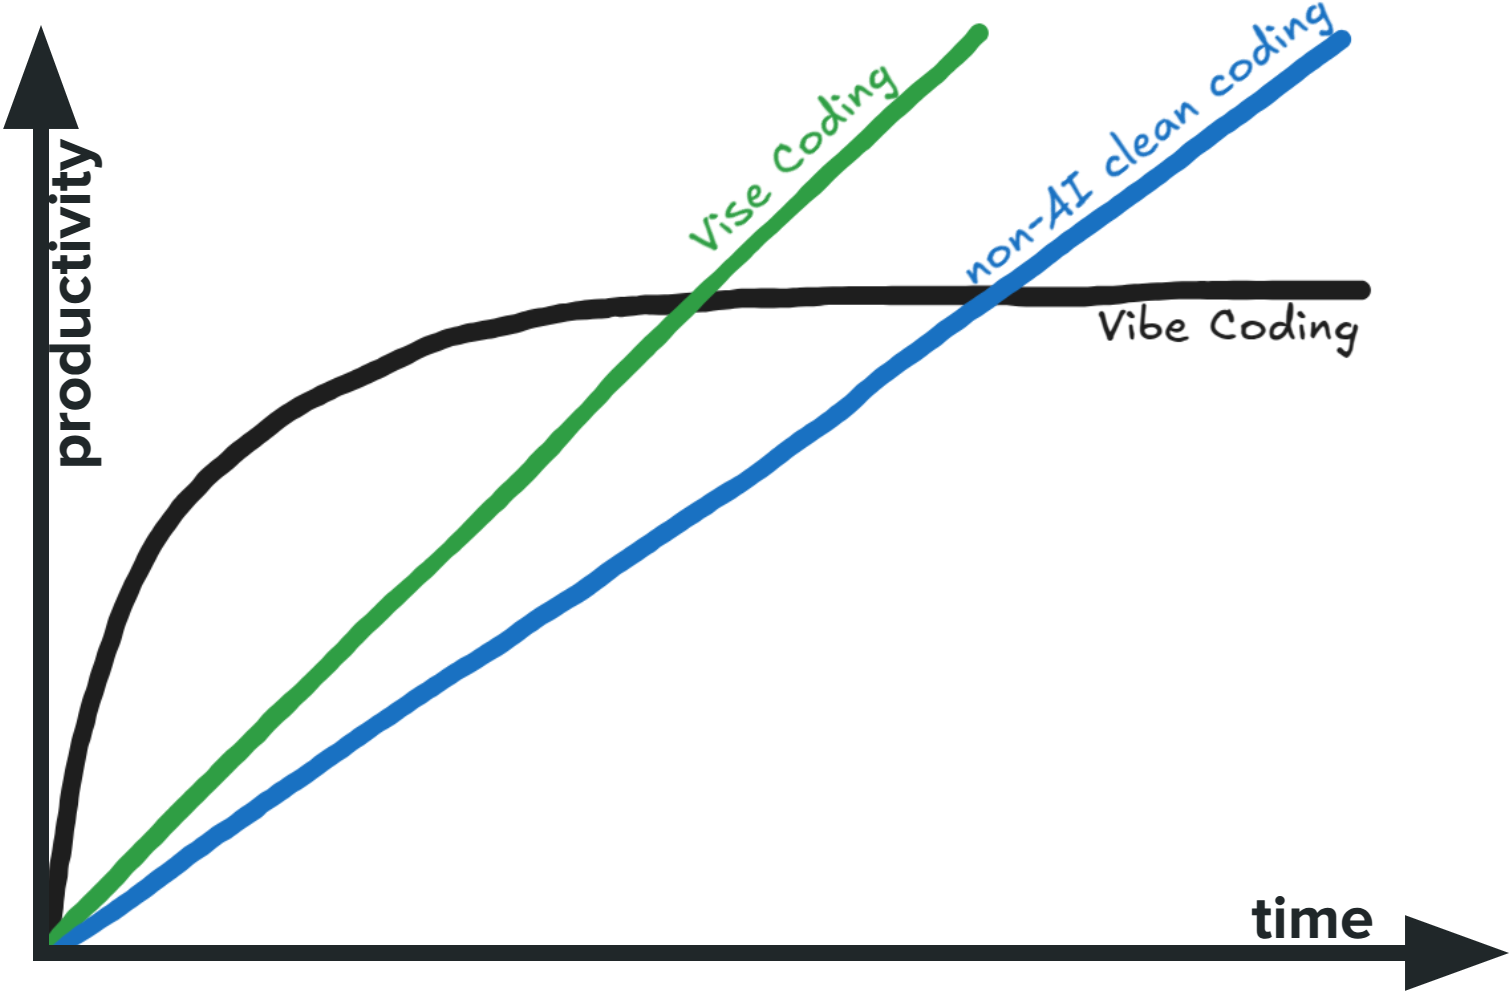
\includegraphics[width=0.47\textwidth]{figures/vibe_vise_non_ai_v2}
  \vspace{-5mm}
\caption{Vibe Coding vs Vise Coding productivity}
\label{fig:vibevise}
\end{center}
\end{figure}

\newpage 
%\hbadness=2000
%\printbibliography
\bibliographystyle{plain}
\bibliography{vise}

\end{document}
